\documentclass{beamer}
%\documentclass[notes=only]{beamer}   % only notes
\usetheme[progressbar=foot]{metropolis}

\setbeamertemplate{frame footer}{\tiny{\inserttitle \textbar \insertauthor \textbar \insertdate}}

% IMPORTS
\usepackage[ngerman]{babel}
\usepackage[utf8]{inputenc}
% \usepackage[T1]{fontenc}
\usepackage{graphicx}	% Einbinden von Grafiken
\usepackage{float}		% figure: [H]
\usepackage{wrapfig}	% figure: [l]
\usepackage{subfigure}
\usepackage{caption}
\usepackage{url}
\usepackage{hyperref}
\usepackage{hepnames}
\usepackage{csquotes}
\usepackage[style=numeric,backend=biber]{biblatex}

% Set bib file
\bibliography{literature}

% Removes icon in bibliography
\setbeamertemplate{bibliography item}{}

% Custom colors
\usepackage{xcolor}
\definecolor{deepblue}{RGB}{46,206,227}
\definecolor{deepred}{RGB}{245,20,66}
\definecolor{deepgreen}{RGB}{98,213,51}
\definecolor{deepgrey}{RGB}{183,183,183}
\definecolor{deepyellow}{RGB}{222,203,80}
\definecolor{commentgreen}{RGB}{78,139,70}

\usepackage{listings}

\lstset{ 
language=Python,
basicstyle=\fontsize{9}{9}\ttfamily,
otherkeywords={self},                   % Add keywords here
keywordstyle=\ttfamily\color{deepblue},
emph={MyClass,__init__},                % Custom highlighting
emphstyle=\ttfamily\color{deepred},     % Custom highlighting style
stringstyle=\color{deepgreen},
commentstyle=\color{commentgreen},      % comment style
frame=trbl,                             % Any extra options here
tabsize=2,
showstringspaces=false,
breaklines=true,
numbers=left,
extendedchars=false,
escapeinside=”
}

\title{Grundkurs: Programmieren}
\subtitle{Einführung in grundlegende Programmierkonzepte mit Python}
\date{WS 17/18}
\author[CS]{Christoph Sonntag}
\institute{Universität Passau}
\subject{Computer Science}

\begin{document}
\maketitle

\section{Einführung in die Programmierung}

\begin{frame}{Erwartungen und Vorkenntnisse}
    \begin{itemize}
        \item Erwartungen an den Kurs?
        \item Bereits Programmierkenntnisse aus Schule/Universität?
        \item Kursziele 
            \begin{itemize}
                \item grundlegendes Verständnis
                \item ``mit Informatikern reden können"
                \item Angst nehmen
            \end{itemize}
    \end{itemize}
\end{frame}

\begin{frame}{Die Programmiersprache Python}
\begin{columns}
    \column{0.5\textwidth}
    \begin{itemize}
        \item Warum Python?
            \begin{itemize}
                \item flache Lernkurve, sehenswerte Ergebnisse bereits nach dem ersten Tag
                \item verankert in Forschung und Wirtschaft
                \item der englischen Sprache sehr änhlich
            \end{itemize}
    \end{itemize}
    \column{0.5\textwidth}
    \centering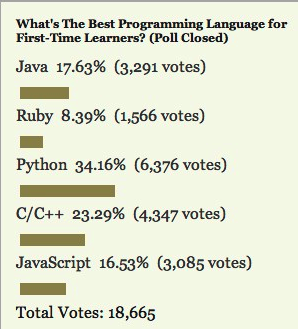
\includegraphics[scale=0.5]{images/best_lang} 
    \hyperlink{https://lifehacker.com/five-best-programming-languages-for-first-time-learners-1494256243}{\tiny{Quelle: lifehacker.com}}
\end{columns}
\end{frame}

\defverbatim{\pythonenglish}{%
\begin{lstlisting}[frame=none,basicstyle=\fontsize{9}{11}\ttfamily]
languages = ["C", "C++", "Java", "Python", "Fortran"]
modern_languages = \ 
    list((x for x in languages if x is not "Fortran"))
\end{lstlisting}
}
\begin{frame}[standout]
    \pythonenglish
\end{frame}


\begin{frame}{Installieren von Python}
    \begin{itemize}
        \item Python 3.6.3 unter \url{https://www.python.org/downloads/} herunterladen 
        und ausführen
        \item Zum `PATH' hinzufügen und `\dots for all users' deaktivieren
    \end{itemize}
    \begin{figure}
        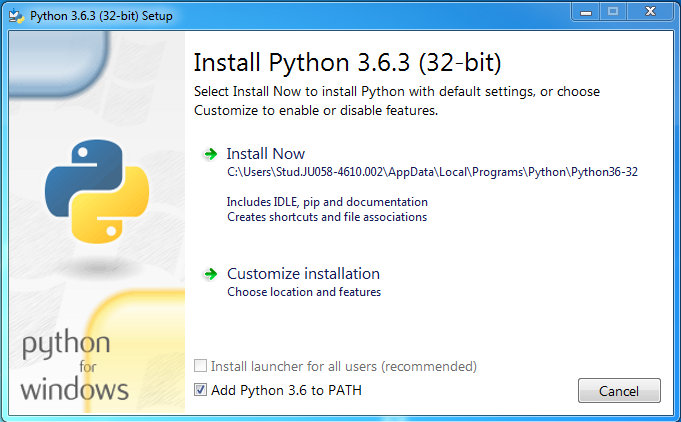
\includegraphics[scale=0.4]{images/python_install} 
    \end{figure}
\end{frame}


\begin{frame}[fragile]{Hello World}
    \begin{lstlisting}
    print("Hello World!")
    \end{lstlisting}
    \begin{itemize}
        \item IDLE suchen und starten
        \item eintippen und mit Enter ausführen
        \item gibt den Text (String) `Hello World!' auf der Konsole aus
    \end{itemize}
    \begin{exampleblock}{Glückwunsch}
    Ihr habt gerade euer erstes Code-Fragment geschrieben und ausgeführt!
    \end{exampleblock}
\end{frame}

\begin{frame}[fragile]{Hello World}
    \begin{block}{Aufgabe 1}
        Erweitere das Programm so, dass der \texttt{String} `Hello World'
        6-mal auf der Konsole ausgegeben wird.
    \end{block}
    \pause{}
    \begin{exampleblock}{Lösung}
        \begin{lstlisting}
print("Hello World")
print("Hello World")
print("Hello World")
print("Hello World")
print("Hello World")
print("Hello World")
        \end{lstlisting}
    \end{exampleblock}
\end{frame}

\begin{frame}[fragile]{Hello World}
    \begin{itemize}
        \item \texttt{sleep(num)}
            \begin{itemize}
                \item stoppt die Ausführung des Programms für \texttt{num} Sekunden
                \item ist nicht Teil des Standard-Pythons, sondern muss importiert 
                    werden. \lstinline[columns=fixed]{from time import sleep}
            \end{itemize}
    \end{itemize}
    \pause{}
    \begin{block}{Aufgabe 2}
        Lass das Programm einen realistischen Monolog ausführen. 
        Verwende hierzu \texttt{sleep}
    \end{block}
    \pause{}
    \begin{exampleblock}{Lösung}
        \begin{lstlisting}
from time import sleep

print("Hey, it's James!")
sleep(2)
print("I'm working on a ChatBot right now")
sleep(3)
...
        \end{lstlisting}
    \end{exampleblock}

\end{frame}


\begin{frame}{Entwicklungsumgebung einrichten}
    \begin{alertblock}{Achtung}
        Word, TextEdit, Notepad, oder Wordpad sind Textverarbeitungsprogramme, keine 
        Quelltext-Editoren und schon gar keine Entwicklungsumgebungen
    \end{alertblock}
    \pause{}
    \begin{itemize}
        \item Editoren wie \texttt{Sublime Text, Atom} oder \texttt{IDLE} sind 
        für uns ausreichend
        \item große IDE's wie \texttt{Eclipse}, \texttt{IntelliJ} oder \texttt{PyCharm} 
        bieten weitere Funktionen
    \end{itemize}
\end{frame}

\begin{frame}{Entwicklungsumgebung einrichten}
    \begin{itemize}
        \item Pythonprogramme in IDLE schreiben und ausführen
            \begin{enumerate}
                \item\texttt{Datei} $>$ \texttt{Neue Datei}
                \item geeigneten Speicherort aussuchen, bspws. \texttt{Dokumente/GrundkursProgrammieren/helloworld.py}
                \item Programm schreiben\dots
                \item Programm unter \texttt{Run} $>$ \texttt{Run Module} ausführen oder F5 drücken
            \end{enumerate}
    \end{itemize}
\end{frame}


\begin{frame}[fragile]{Typen und Variablen}
Wir haben ganz unbewusst bereits zwei Datentypen benutzt
\begin{itemize}
    \item \texttt{String, str}: 
    \begin{lstlisting}
print("Ich bin vom Typ String, eine Reihe von Zeichen")
    \end{lstlisting}
    \item \texttt{Integer, int}: 
    \begin{lstlisting}
sleep(3)   # 3 ist ein Integer
    \end{lstlisting}
\end{itemize}
\end{frame}

\begin{frame}[fragile]{Typen und Variablen}
\begin{itemize}
    \item Wahrheitswert (Boolean, bool): 
    \begin{lstlisting}
wahr = True
falsch = False
    \end{lstlisting}
    \item Gleitkommazahlen (Float, float):
    \begin{lstlisting}
pi = 3.1415
    \end{lstlisting}
    \item In Python gibt es sogar komplexe Zahlen \texttt{complex}:
    \begin{lstlisting}
a = complex('3+5j')
    \end{lstlisting}

\end{itemize}
\end{frame}

\begin{frame}[fragile]{Typen und Variablen}
\begin{itemize}
    \item Zuweisung von Variablen mit dem Zuweisungsoperator \texttt{=}
    \begin{lstlisting}
a = 5
b = 3.14
c = "Hallo Grundkurs:Programmieren"
    \end{lstlisting}
    \item der Variable kann auch das Ergebnis einer Operation zugewiesen werden
    \begin{lstlisting}
a = 1000
b = 200
percent = b / a * 100
    \end{lstlisting}
    \item mehrfache Zuweisung 
    \begin{lstlisting}
a, b, c = 5, 3.14, "Hallo Grundkurs:Programmieren"
x = y = z = 42
    \end{lstlisting}
\end{itemize}
\end{frame}


\begin{frame}[fragile]{Typsicherheit}
 \begin{itemize}
    \item streng-getypte Sprachen: \textbf{Java}, C/C++, \dots
    \begin{lstlisting}
int x = 42
float pi = 3.14
String greeting = "Hallo Grundkurs:Programmieren"
boolean truth = true
    \end{lstlisting}
    \item dynamisch (schwach) getypte Sprachen: \textbf{Python}, Javascript
    \begin{lstlisting}
x = 42
pi = 3.14
greeting = "Hey there"
truth = True
    \end{lstlisting}
\end{itemize}   
\end{frame}

\begin{frame}[fragile]{Typsicherheit}
\begin{block}{Aufgabe}
Gib folgende Ausdrücke in den Python Interpreter ein:
\begin{lstlisting}
>>> 3 + 3.14
>>> "Mein Alter: " + 5
>>> True + 1
\end{lstlisting}
\end{block}
\pause{}
\begin{exampleblock}{True + 1 == 2?}
Intern werden die Keywords \lstinline{True} und \lstinline{False} auf die 
Werte \texttt{1} und \texttt{0} vom Typ \texttt{int} abgebildet.
\end{exampleblock}

\end{frame}


\begin{frame}[fragile]{Typen und Variablen}
    Die \lstinline{input()} Funktion nimmt Benutzereingaben auf der Kommandozeile 
    entgegen und gibt sie als String zurück. Du brauchst kein zusätzliches Modul importieren.
    \begin{block}{Aufgabe}
       Lasse dich von deinem Programm begrüßen, indem du mit \texttt{input} deine 
       Eingabe in einer Variable speicherst.
    \end{block}
    \pause{}
    \begin{exampleblock}{Lösung}
        \begin{lstlisting}
>>> name = input()
'Christoph'
>>> print("Hallo " + name)
        \end{lstlisting}
    \end{exampleblock}
\end{frame}

\begin{frame}[fragile]{Typconversion}
    \begin{alertblock}{Achtung}
    Die \lstinline{input()} Funktion interpretiert jede Benutzereingabe
    als \texttt{String}. Wenn man Zahlen aufnehmen will, muss der Typ
    `gecastet' werden, d.h. `umgewandelt'.
    \begin{itemize}
        \item \lstinline{int()}: Castet zu int.
        \item \lstinline{str()}: Castet zu String.
    \end{itemize}
    Was passiert bei \lstinline{int("HalloWelt")}?
    \pause{}
    Ein \texttt{ValueError} wird geworfen. (Exception handling nicht 
    in diesem Kurs)
    \end{alertblock}
\end{frame}


\begin{frame}{Programmiersprachen}
    \begin{itemize}
        \item Unterscheidungsmerkmale
            \begin{itemize}
                \item Programmierparadigma: imperativ, funktional oder objektorientiert
                \item Typsicherheit
                \item kompiliert vs. interpretiert
                \item allgemein vs. domänenspezifisch
                \item hardwarenah vs. höhere Programmiersprachen
            \end{itemize}
    \end{itemize}
\end{frame}

\begin{frame}[fragile]{Programmiersprachen}
    \begin{itemize}
        \item Imperative Programmiersprachen: C/C++, C\#, Java \dots
        \item Funktionale Programmiersprachen: SQL, Haskell, Erlang, (Scala) \dots
        \item Objektorientierte Programmiersprachen: C++, C\#, Java, Javascript, PHP, Python \dots
    \end{itemize}
\end{frame}

\begin{frame}[fragile]{Imperative Sprachen (C/C++, C\#, Python, Java, \dots)}
    \begin{itemize}
        \item ältestes Programmierparadigma
        \item große Verbreitung in der Industrie
        \item besteht aus Befehlen (lat. imperare = befehlen)
        \item Abarbeiten der Befehle `Schritt für Schritt'
        \item sagt einem Computer, `wie' er etwas tun soll
    \end{itemize}
    \begin{lstlisting}
print("Hey, whats' up?")
sleep(3)
print("Learning Python right now")
sleep(2)
    \end{lstlisting}
    \begin{itemize}
        \item Verwendung
            \begin{itemize}
                \item `Standard-Software', hardwarenahe Entwicklung
            \end{itemize}
    \end{itemize}
\end{frame}

\begin{frame}[fragile]{Funktionale Sprachen (Haskell, Erlang, SQL, Lisp, \dots)}
    \begin{itemize}
       \item vergleichsweise modern
       \item sagt einem Computer, `was' das Ergebnis sein soll
       \item SELECT name FROM students WHERE major=‘law’ AND semester=‘1’;
       \item Verwendung
        \begin{itemize}
            \item akademische Zwecke
            \item sicherheitskritische und \dots
            \item hoch performante Anwendungen
        \end{itemize}
    \end{itemize}
    \begin{lstlisting}
square :: [Int] -> [Int]
square a = [2*x | x <- a]
    \end{lstlisting}
\end{frame}

\defverbatim{\impvsfunc}{%
\begin{lstlisting}[frame=none,numbers=none,basicstyle=\fontsize{15}{18}\ttfamily]
            x = x + 1
\end{lstlisting}
}
\begin{frame}[standout]
    \impvsfunc
\end{frame}

\begin{frame}[fragile]{Objektorientierte Sprachen (Java, Python, C++, C\#, \dots)}
    \begin{itemize}
       \item starke Verbreitung
       \item Abbilden der realen Welt der Dinge auf Objekte
       \item Klasse: Bauplan eines Objekts bestehend aus Eigenschaften (Attributen) und Methoden
       \item Vererbung möglich
       \item Verwendung
        \begin{itemize}
            \item Standard-Software
            \item Modellierung realer Projekte(Unternehmen, Mitarbeiter, Kunden, Waren, \dots)
            \item große Projekte ($\rightarrow$ Planung durch Klassendiagramme)
        \end{itemize}
    \end{itemize}
\end{frame}

\begin{frame}[fragile]{Objektorientierung: Beispiel}
    \begin{lstlisting}
class Konto:
    def __init__(self, name, nr):
        self.inhaber = name
        self.kontonummer = nr
        self.kontostand = 0
    def einzahlen(self, betrag):
        self.kontostand = kontostand + betrag
    def auszahlen(self, betrag):
        self.kontostand = kontostand - betrag
    def ueberweisen(self, ziel, betrag): 
        ziel.einzahlen(self.betrag)
        self.auszahlen(betrag)
    def kontostand(self):
        return self.kontostand

class Unternehmenskonto(Konto):
    def erhalteBonus(self, bonus):
        self.kontostand = kontostand + bonus
    \end{lstlisting}
\end{frame}

\begin{frame}[fragile]{Kompilierte und Interpretierte Sprachen}
    \begin{itemize}
        \item kompilierte Sprachen (Java, C/C++, C\#, \dots):
        \begin{itemize}
            \item Übersetzung des (kompletten) Programmcodes in Maschienencode
            \item dann Ausführung des Maschinencodes
        \end{itemize}
        \item interpretierte Sprachen (Python, Lisp, PHP, JavaScript, \dots):
        \begin{itemize}
            \item Übersetzung einer einzelnen Programmanweisung
            \item Ausführung dieser Anweisung
            \item Übersetzung der nächsten Anweisung
        \end{itemize}
    \end{itemize}
\end{frame}

\begin{frame}[fragile]{Hardwarenahe und höhere Sprachen}
\begin{itemize}
    \item hardwarenah: abhängig von der Bauweise des Prozessors
    \item höhere Sprachen: von der Bauweise abstrahiert (\texttt{print(), sleep()})
\end{itemize}
\begin{columns}
    \column{0.3\textwidth}
    \begin{lstlisting}
.START ST
  ST: MOV R1,#2
      MOV R2,#1
  M1: CMP R2,#20
      BGT M2
      MUL R1,R2
      INI R2
      JMP M1
  M2: JSR PRINT
      .END
    \end{lstlisting}
    \column{0.3\textwidth}
    \begin{lstlisting}

a = 2;
i = 1;
# compare i == 20
# if True, jump to M2
a = a*i;
i++;
# jump to M1
print(a)
    \end{lstlisting}
    \column{0.3\textwidth}
    \begin{lstlisting}
a = 2;
for i in range(1, 20) {


    a = a*i;
}
 
 
print(a);

    \end{lstlisting}
\end{columns}
\end{frame}

\begin{frame}{Populäre Programmiersprachen}
    \begin{itemize}
        \item C++
            \begin{itemize}
                \item imperativ, objektorientiert, typsicher, kompiliert, allgemein,
                höhere Sprache (dennoch hardwarenah)
                \item große Verwendung in hocheffizienten Systemen 
                (Betriebssysteme, Grafikberechnungen, Computerspiele, \dots)
                \item Erweiterung von C mit Objektorientierung
            \end{itemize}
        \item Java
            \begin{itemize}
                \item imperativ, objektorientiert, typsicher, kompiliert, allgemein
                \item im bayrischen Lehrplan und an vielen Universitäten 
                `erste' Sprache
                \item ebenfalls große Verbreitung
            \end{itemize}
        \item Python
            \begin{itemize}
                \item (imperativ), (funktional), objektorientiert, 
                dynamisch getypt, interpretiert, allgemein
                \item große Verbreitung auch gerade im akademischen Umfeld, 
                Web, Machine Learning und Data Science
            \end{itemize}
    \end{itemize}
\end{frame}


\begin{frame}[fragile]{Exkurs: Kommentierung, Lesbarkeit und Wartbarkeit}
    \begin{lstlisting}
"""
Das ist ein Kommentar, der sich ueber mehrere Zeilen
erstreckt und in der Regel in ganzen Saetzen spricht.
Das Ziel ist etwas ausfuehrlich zu erklaeren.
"""
print("Wozu Kommentare?") # stellt eine Frage
    \end{lstlisting}
    \begin{itemize}
        \item Zeilen, die mit '\# ' beginnen, sind einzeilige Kommentare
        \item mehrzeilige Kommentare häufig bei Klassen ($\rightarrow$ automatische 
        Erzeugung von Dokumentationen)
        \item werden nicht ausgeführt
        \item zur Erläuterung von Programmcode
        \item Aufwendig, aber sehr wichtig! (Lesbarkeit, Wartbarkeit)
    \end{itemize}
\end{frame}

\begin{frame}[fragile]{Exkurs: Kommentierung, Lesbarkeit und Wartbarkeit}
    \begin{lstlisting}
# set the value of the age to an integer with the value 32
age = 32
    \end{lstlisting}
    \pause{}
    \begin{alertblock}{Schlechtes Beispiel}
    Unnötige Erklärung einer offensichtlichen Sache
    \end{alertblock}
\end{frame}

\begin{frame}[fragile]{Exkurs: Kommentierung, Lesbarkeit und Wartbarkeit}
    \begin{lstlisting}
def addSetEntry(set, value):
  """ 
   Don't return set.add because it's not chainable in Internet Explorer 11.
  """ 
  set.add(value)    
  return set
    \end{lstlisting}
    \pause{}
    \begin{lstlisting}
"""
This code sucks, you know it and I know it.  
Move on and call me an idiot later.
"""
    \end{lstlisting}
    \pause{}
    \begin{lstlisting}
# Class used to workaround Richard being a f***ing idiot
    \end{lstlisting}
\end{frame}


\begin{frame}[fragile]{Datenstrukturen: Listen}
Listen sind praktische Datenstrukturen, um eine Folge von Werten zu 
speichern oder zu erzeugen.
Oft reichen Integer, Float und String Datentypen nicht aus. Meist wissen wir nämlich im Voraus nicht, 
wie viele Datensätze gespeichert werden sollen.
\pause{}
\begin{lstlisting}
zahlen = [1, 2, 3, 4, 5, 6]
texte = ["Hallo", "Welt", ".", ["Grundkurs", "Programmieren"]]
\end{lstlisting}

\begin{lstlisting}
>>> zahlen[3]
4
>>> texte[0]
"Hallo"
>>> texte[3]
["Grundkurs", "Programmieren"]
\end{lstlisting}
\end{frame}

\begin{frame}[fragile]{Datenstrukturen: Listen}
Die Liste bietet eine große Anzahl an Methoden (Funktionen), die auf ihnen
ausgeführt werden können.
\begin{block}{Aufgabe}
\begin{lstlisting}
>>> liste = ["Grundkurs", "Programmieren", 42, "Pie", 3.14]

>>> liste[2] = 99
>>> len(liste)
>>> liste.append("Passau")
>>> liste.extend([4, 5, 3.14])
>>> liste.insert(2, "Falke")
>>> liste.count(3.14)
>>> liste.index(3.14)
>>> liste.remove(3.14)
>>> liste.pop()
>>> liste.reverse()
>>> sum([1,3,5])
>>> max([1,3,5])
\end{lstlisting}
\end{block}
\end{frame}

\begin{frame}[fragile]{Datenstrukturen: Listen}
\begin{block}{Aufgabe}
Versuche zu erraten, was die Ausgabe dieses Programms ist.
\end{block}

\begin{lstlisting}
liste_a = ["Hallo", "schoenes", "Wetter"]
liste_b = liste_a

liste_b[1] = "schlechtes"

print(liste_a[0], liste_a[1], liste_a[2])  
\end{lstlisting}
\pause{}
\begin{exampleblock}{Lösung}
    \texttt{Hallo schlechtes Wetter}
\end{exampleblock}
\end{frame}

\begin{frame}[fragile]{Datenstrukturen: Listen}
\begin{block}{Aufgabe: Notendurchschnitt}
Schreibe ein Programm, dass drei Prüfungs-Noten einliest, in einer
Liste speichert und dir nach jeder Eingabe den Durschnitt errechnet. 
\end{block}
\begin{lstlisting}

\end{lstlisting}
\pause{}
\begin{exampleblock}{Lösung}
siehe Beamer
\end{exampleblock}
\end{frame}


\begin{frame}{Syntax in Python}
\begin{itemize}
    \item der Code wird durch Einrückungen (Tabs) strukturiert (vgl. \texttt{for}-Schleife)
    \item runde Klammern () sind meist für Parameter (\lstinline{print("Hier der Text")}) 
    \item eckige Klammern [] sind meist für `listenartige' Datenstrukturen (Arrays, Listen in Python)
    \item Leerzeichen und Zeilenumbrüche sind meist optional, verbessern aber die Lesbarkeit des Programms
    \item Groß- und Kleinschreibung muss meist beachtet werden
\end{itemize}
\end{frame}

\begin{frame}{Konventionen für lesbareren Code}
Damit Code einheitlich gut lesbar ist, gibt es für Programmiersprachen 
`Coding Conventions', die zwar nicht erfüllt werden \textit{müssen}, aber 
einen guten Eindruck hinterlassen und zur besseren Lesbarkeit beitragen. \\
Auszug (\textit{PEP8}): 
\begin{itemize}
    \item Variablen- und Funktionsnamen klein und wenn nötig \\ mit \_ schreiben 
    \item Eine Einrückungsebene in Python entspricht genau 4 Leerzeichen (keine Tabulatorzeichen) 
    \item Am Anfang jeder Python-Datei steht ein Doc-String (Kommentar), der kurz den Inhalt der Datei bescheibt
    \item \dots bei Funktionen auch
\end{itemize}
\end{frame}


\begin{frame}[fragile]{Die \texttt{for}-Schleife}
\begin{block}{Aufgabe}
    Schreibe ein Programm, dass von 1 bis 100 zählt.
    \begin{lstlisting}
print("Ich kann uebrigens bis 100 zaehlen ... ;-)")
...
    \end{lstlisting}
\end{block}
\pause{}
\begin{exampleblock}{Lösungsvariante 1}
    \begin{lstlisting}
print(1)
print(2)
print(3)
print(4)
print(5)
print(6)
print(7)
...
    \end{lstlisting}
\end{exampleblock}
\end{frame}

\begin{frame}[fragile]{Die \texttt{for}-Schleife}
Vereinfachte weniger schreibintensive Variante:
\begin{exampleblock}{Lösungsvariante 2}
    \begin{lstlisting}
for i in range(1, 100):
    print(i)
    \end{lstlisting}
\end{exampleblock}
\begin{itemize}
    \item gibt die Werte von 1 bis 99 aus
    \item Die Variable \texttt{i} nimmt hierbei nacheinander (d.h.\ nach jedem Schleifendurchlauf) jeden Wert 
        aus der angegebenen \texttt{range} einmal an.
    \item \texttt{i} ist ein beliebige Variable, das heißt, man kann ihr auch einen anderen Namen geben
    \pause{} 
    \item gib in den Interpreter \texttt{help()} ein, um genaueres über 
    eine Funktion zu erfahren. 
    \pause{}
    \item aus der Dokumentation: \texttt{range(i, j) produces i, i+1, i+2, ..., j-1.}
\end{itemize}
\end{frame}

\begin{frame}[fragile]{Die \texttt{for}-Schleife}
\begin{itemize}
    \item Andere Sprachen erzeugen kein 'extra Objekt', sondern zählen eine 
    Variable hoch
    \item genauer: setzt $i=1$, addiert in jedem Schritt 1 auf, 
    solange $i < 100$ ist. 
\end{itemize}
\begin{lstlisting}[language=Java]
for(int i=1, i < 100, i++) {
    // gib i aus
}
\end{lstlisting}
\end{frame}

\begin{frame}[fragile]{Die \texttt{for}-Schleife}
\begin{block}{Aufgabe}
Ändere das Programm von gerade eben so, dass wirklich bis 100 gezählt wird.
\end{block}
\pause{}
\begin{exampleblock}{Lösung}
\begin{lstlisting}
for i in range(1, 101):
    print(i)
\end{lstlisting}
\end{exampleblock}
\end{frame}

\begin{frame}[fragile]{Die \texttt{for}-Schleife}
\begin{block}{Aufgabe}
Bildet 2-3er Gruppen und schreibt ein Programm, dass von 10 bis 0 herunterzählt.
\textit{Hinweis:} Verwendet zum pausieren zwischen den Zahlen wieder \texttt{sleep()}.
\lstinline{from time import sleep} nicht vergessen.
\end{block}
\pause{}
\begin{exampleblock}{Lösung}
    siehe Beamer
\end{exampleblock}
\end{frame}


\begin{frame}[fragile]{Gültigkeit von Variablen - der Scope}
    \begin{block}{Aufgabe}
    Schreibe ein Programm, dass sich dem Benutzer vorstellt und anschließend
    nach Namen und Alter fragt. Verwende hierzu die 
    Funktionen \lstinline{input()} und \lstinline{print()}. (Wenn du willst auch
    \lstinline{sleep()}).
    \end{block}

    \begin{alertblock}{Anfang}
    \begin{lstlisting}
name = "James"
print("Hey, i'm " + name + " and what's you're name?")
...
    \end{lstlisting}
    \end{alertblock}

    \pause{}

    \begin{exampleblock}{mögliche Lösung}
    \begin{lstlisting}
...
name = input() # ueberschreibt die vorige Variable 
sleep(2)
print("Ahh, so you're " + name)
...
    \end{lstlisting}
    \end{exampleblock}
\end{frame}


\begin{frame}[fragile]{logische Operatoren}
Den Zuweisungsoperator \texttt{=} haben wir unbewusst bereits kennengelernt. 
Er weißt einem Wert bspws.\ einen Namen zu (\lstinline{x = 42}). Die Operatoren 
\texttt{+}, \texttt{-}, \texttt{/} oder \texttt{*} verwenden wir intuitiv.\\

Zum besseren Vergleichen brauchen wir weitere Operatoren:
\begin{itemize}
    \item \texttt{==}: prüft zwei Werte auf Gleichheit
    \item \texttt{!=}: prüft zwei Werte auf Ungleichheit
    \item \texttt{>}: größer
    \item \texttt{<}: kleiner (vgl.\ for-Schleife)
    \item kleiner-gleich?
    \pause{}
    \item \texttt{<=, >=}, kleiner-gleich, größer-gleich
    \item \texttt{and}: logisches `Und'
    \item \texttt{or}: logisches `Oder'
    \item \texttt{not}: verneint einen Ausdruck
\end{itemize}
\end{frame}

\begin{frame}[fragile]{logische Operatoren}
Was ergeben folgende Ausdrücke? Überprüfe sie mit dem Python Interpreter.

\begin{lstlisting} 
3 > 4 
\end{lstlisting}

\begin{lstlisting} 
6 != 7
\end{lstlisting}

\begin{lstlisting} 
"Hallo" < "Hallo Welt!"
\end{lstlisting}

\begin{lstlisting} 
"Hallo" == "Hallo Welt"
\end{lstlisting}

\begin{lstlisting} 
"Hallo Welt" == "Hallo" and 3 > 4
\end{lstlisting}

\begin{lstlisting} 
not not 5 == 5
\end{lstlisting}

\end{frame}


\begin{frame}{Recap}
    \begin{block}{Aufgabe}
        Schreibe ein Programm, welches vom Benutzer 6 Zahlen einliest, diese 
        in einer Liste speichert und anschließend das Maximum ausgibt.
    \end{block}
\end{frame}

\begin{frame}[fragile]{Recap}
    \begin{exampleblock}{Lösung}
        \begin{lstlisting}
numbers = []
for i in range(0,7):
    input_num = int(input())
    numbers.append(input_num)

maximum = max(numbers)
print("Maximum: " + str(maximum))
# print("Maximum: \%d" \% maximum)
        \end{lstlisting}
    \end{exampleblock}
\end{frame}

\begin{frame}[fragile]{Bedingte Ausführung}
Hilft uns beim strukturieren des Programms in verschiedene Richtungen.
Struktur:

\begin{lstlisting}
if Bedingung:
    # Programmcode
else:
    # alternativer Programmcode, wenn Bedingung nicht zutrifft
\end{lstlisting}
\pause{}
\begin{lstlisting}
zahl = input()

if zahl > 10:
    print("Die Zahl ist > 10.")
else:
    print("Die Zahl ist < 10.")
\end{lstlisting}
\end{frame}

\begin{frame}[fragile]{Bedingte Ausführung}
    \begin{block}{Aufgabe}
        Schreibe eine Programm, das zwei Zahlen vom Benutzer einliest, testet, 
        ob die erste durch die zweite Zahl teilbar ist und das Ergebnis ausgibt.
        \pause{}
        \begin{lstlisting}
zahl1 = int(input("Erste Zahl: "))
zahl2 = int(input("Zweite Zahl: "))

if zahl1 ‘%‘ zahl2 == 0:
    print("Zahl 1 ist durch die Zweite teilbar!")
else: 
    print("Leider kann man die Zahlen nicht ohne Rest teilen")
        \end{lstlisting}
    \end{block}
\end{frame}

\begin{frame}[fragile]{Bedingte Ausführung}
Mehrere Bedingungen?
\pause{}
\begin{lstlisting}
zahl = input()

if zahl > 10:
    print("Die Zahl ist > 10.")
elif zahl > 100:
    print("Die Zahl ist > 100.")
else:
    print("Die Zahl ist < 10.")

\end{lstlisting}
\end{frame}

\begin{frame}{Bedingte Ausführung}
    \begin{block}{Aufgabe}
        Schreibe ein Programm, dass ein eingegebenes Hundealter in Menschenjahre umrechnet.
        \begin{itemize}
            \item 1 Hundejahr $=$ 14 Jahre
            \item 2 Hundejahre $=$ 22 Jahre
            \item Über 2 Jahren $= 22 + (Alter -2) * 5$
        \end{itemize}
    \end{block}
\end{frame}

\begin{frame}[fragile]{Bedingte Ausführung}
    \begin{exampleblock}{Lösung}
        \begin{lstlisting}
age = int(input("Alter des Hundes: "))
if age < 0:
    print("Das stimmt wohl kaum!")
elif age == 1:
    print("entspricht ca. 14 Jahren")
elif age == 2:
    print("entspricht ca. 22 Jahren")
elif age > 2:
    human = 22 + (age -2)*5
    print("entspricht ca. " + str(human) + "Jahren")
        \end{lstlisting}
    \end{exampleblock}
\end{frame}


\begin{frame}{Bedingte Ausführung}
    \begin{block}{Aufgabe}
        Schreibe ein Programm, das errechnet, ob ein eingegebenes Jahr ein
        Schaltjahr ist.
        \begin{itemize}
            \item durch 400 teilbar: ist ein Schaltjahr
            \item durch 100 teilbar: ist kein Schaltjahr
            \item falls durch 4 teilbar: ist ein Schaltjahr
        \end{itemize}
    \end{block}
    \pause{}
    \begin{exampleblock}{gemeinsame Lösung}
    siehe Beamer
    \end{exampleblock}
\end{frame}



\begin{frame}{Exkurs: Projekt Dimensionen}
\begin{itemize}
    \item Programme in der Regel wesentlich länger als 100 Zeilen
    \pause{}
    \item Metrik zur Aufwandsberechnung z.B. Lines of Code. (LOC, SLOC)
        \begin{itemize}
            \item Windows XP: ca. 40 Mio. SLOC
            \item Mac OS X Tiger: ca. 86 Mio. SLOC
        \end{itemize}
    \pause{}
    \item nicht zwangsläufig Rückschlüsse auf die Komplexität oder Funktionalität
\end{itemize}
\end{frame}

\iffalse
\begin{frame}{Exkurs: Projekt Dimensionen}
\begin{itemize}
    \item Projektgröße: Als Maßstab gilt meist das Budget. „Kleine“ Projekte sind oft
auch einfach und flach strukturiert. Hier sollte minimaler Aufwand betrieben
werden.
    \pause{}
    \item Projektrisiken: Hohe Risiken verlangen nach sorgfältigem Risikomanagement.
    \pause{}
    \item Komplexität: Hohe Komplexität stellt Anforderungen an die Dokumentation,
Planung und Kontrolle. Man sollte prüfen, ob eine Aufteilung des Projektes
möglich ist.
    \pause{}
    \item Projektdauer: „Langläufer“ erfordern gute Dokumentation und eine laufende
Überprüfung des zugrunde liegenden „Business Case“.
\end{itemize}
\end{frame}

\begin{frame}{Exkurs: Projekt Dimensionen}
\begin{itemize}
    \item Bedeutung für das Unternehmen: Eine hohe Bedeutung ist verbunden mit besonderen Informationspflichten in das Management und hohen Erwartungen
bzgl. der Termineinhaltung.
    \pause{}
    \item Auftraggeber (intern / extern): Externe Kundenprojekte haben hohe Anforderungen
an die Leistungsdokumentation, ohne die z.B. keine Abrechnung oder
Leistungsabnahme möglich ist.
    \pause{}
    \item Innovationsgrad: „Standardprojekte“ sind etabliert und werden nach einfachen
Standards abgewickelt.
    \pause{}
    \item Projektphasen: Eine solide Projektdefinition vor dem Projektstart erspart hohen
Aufwand im Projektablauf. Je nach Projektphase sind unterschiedliche Abteilungen
und Mitarbeiter in dem Projekt aktiv. Kritisch sind dabei die Übergaben.
\end{itemize}
\end{frame}
\fi

\begin{frame}[fragile]{Die \texttt{while}-Schleife}
Ähnlich zur \texttt{for}-Schleife mit dem Unterschied, dass nicht `durch eine Liste gelaufen' wird, 
sondern die Schleife immer wiederholt wird, solange die Bedingung wahr ist.

    \begin{lstlisting}
while Bedingung:
    # Programmcode

# ausserhalb der Schleife
    \end{lstlisting}
\end{frame}

\begin{frame}{Die \texttt{while}-Schleife}
\begin{block}{Aufgabe}
Schreibe ein Programm, welches alle Zahlen von 1 bis 100 auf den Bildschirm schreibt, ohne dafür eine 
for Schleife zu verwenden.
\end{block}
\end{frame}


%\begin{frame}{Die \texttt{while}-Schleife}
%\begin{block}{Aufgabe}
%Die Folge aus Fibonacci-Zahlen wird wie folgt gebildet:
%\begin{itemize}
%    \item Das erste und das zweite Element sind 0 und 1.
%    \item Jedes folgende Element wird gebildet, in dem die letzten zwei Elemente addiert werden.
%\end{itemize}
%Das heisst, die Folge sieht so aus: 0,1,1,2,3,5,8,13,21,34,\dots
%
%Schreibe ein Programm, welches die Fibonacci-Zahlen bis zu einer vom Benutzer gewählten Zahl ausgibt.
%\end{block}
%\end{frame}

%\begin{frame}[fragile]{while-Schleife}
%\begin{exampleblock}{Lösung 1}
%\begin{lstlisting}
%num = 10
%# num = int(input("Bis zu welcher Zahl? "))
%fib1 = 0
%fib2 = 1
%count = 0
%
%if num <= 0:
%   print("Bitte eine positive Zahl eingeben")
%elif num == 1:
%   print("Fibonacci bis zur " + num + "ten Zahl:")
%   print(fib1)
%else:
%    print("Fibonacci bis zur " + num + "ten Zahl:")
%    while count < num:
%	    print(fib1)
%	    fibn = fib1 + fib2
%	    fib1 = fib2
%	    fib2 = fibn
%	    count = count + 1
%        # count += 1
%\end{lstlisting}
%\end{exampleblock}
%\end{frame}

%\begin{frame}[fragile]{while-Schleife}
%\begin{exampleblock}{Lösung 2}
%\begin{lstlisting}
%def fibonacci(n):
%    a = 0
%    b = 1
%    for i in range(0, n):
%        temp = a
%        a = b
%        b = temp + b
%    return a
%\end{lstlisting}
%\end{exampleblock}
%\end{frame}

\begin{frame}{Die \texttt{while}-Schleife}
\begin{block}{Aufgabe: Das kleine 1$\times$1}
Schreibe ein Programm, das den Benutzer `zufällige' 1$\times$1 Rechenaufgaben abfragt und 
die Lösung überprüft. (\lstinline{from random import randint}). Nach jeder Rechenaufgabe 
soll der Benutzer gefragt werden, ob noch eine Aufgabe gestellt werden soll.
\end{block}
\end{frame}

\begin{frame}[fragile]{Die \texttt{while}-Schleife}
\begin{exampleblock}{Lösung}
\begin{lstlisting}
from random import randint

print("Herzlich willkommen zum kleinen EinmalEins Rechner!")
weiter = "Ja"

while weiter == "Ja":
    zahl1 = randint(1, 9)
    zahl2 = randint(1, 9)
    print(str(zahl1) + " x " + str(zahl2))

    loesung = int(input("= "))
    if loesung == zahl1 * zahl2:
        print("Korrekt! Glueckwunsch")
    else:
        print("Leider nicht ganz korrekt. Richtig waere: " + str(zahl1 * zahl2))
    weiter = input("Weiter? (Ja/Nein): ")

print("Vielen Dank!")
\end{lstlisting}
\end{exampleblock}
\end{frame}



% \begin{frame}[fragile]{Dateien lesen und schreiben}
Um Daten, die unsere Programme ausgeben bzw. benötigen, brauchen wir eine 
Möglichkeit, diese zu speichern.
\pause{}
\begin{lstlisting}
daten = open("daten.txt", "r")
for line in daten:
    print(line.rstrip())

daten.close()
\end{lstlisting}

\pause{}

\begin{lstlisting}
zahlen = [1, 2, 3]
daten = open("daten.txt", "w")
for zahl in zahlen:
    daten.write(str(zahl))

daten.close()
\end{lstlisting}
\end{frame}

\begin{frame}[fragile]{Dateien lesen und schreiben}
\begin{block}{Aufgabe}
Baue das Notenprogramm so um, dass die Noten beim Start des Programms aus einer Datei gelesen 
werden und nach Abschluss der Eingabe wieder dort hinein geschrieben werden.
\end{block}
\end{frame}



\begin{frame}[fragile]{Funktionen}
Je größer ein Projekt wird, desto wichtiger ist es den Überblick zu behalten
und evtl. Programmblöcke, die etwas ähnliches machen zusammen zu fassen.

\begin{lstlisting}
def greet():
    print("Hey!")
    print("How are you?")
\end{lstlisting}
\end{frame}

\begin{frame}[fragile]{Funktionen mit Parametern}
Wie die uns bereits bekannten Funktionen \lstinline{print()} und \lstinline{sleep()}
können auch eigene Funktionen Parameter aufnehmen und zurückgeben.

\begin{lstlisting}
def sum(a, b):
    return a + b
\end{lstlisting}

\begin{block}{Aufgabe}
Schreibe eine Funktion, die eine Liste als Parameter nimmt und das Maximum 
zurückgibt.
\end{block}
\end{frame}

\begin{frame}[fragile]{Funktionen mit Parametern und Rückgabewert}
Wie die uns bereits bekannten Funktionen \lstinline{sum()} und \lstinline{max()}
können auch eigene Funktionen Parameter aufnehmen und zurückgeben.

\begin{lstlisting}
def sum(a, b):
    """
    Gibt die Summe zweier Zahlen zurueck.
    """
    return a + b
\end{lstlisting}

\begin{block}{Aufgabe}
Schreibe eine Funktion, die eine Liste als Parameter nimmt und das Maximum 
zurückgibt.
\end{block}
\end{frame}


% \begin{frame}[fragile]{Objektorientierung}
Je größer ein Projekt wird, desto wichtiger ist es, den Überblick 
zu behalten. Funktionen sind eine Art, das Programm übersichtlich zu halten.
Objektorientierung eine weitere.
\pause{}

\begin{lstlisting}
# einfachste Art einer Klasse
class Person:
    pass

james = Person()

james.name = "James"
james.alter = 42
\end{lstlisting}
\end{frame}

\begin{frame}[fragile]{Objektorientierung, die \lstinline{\_\_init\_\_()} methode}

\begin{lstlisting}
class Person():

    def __init__(self):
        self.name = "James"
        self.alter = 42

    def alter_plus_10(self):
        return self.alter + 10

\end{lstlisting}
\end{frame}


\begin{frame}[fragile]{Objektorientierung}
\begin{block}{Aufgabe}
\begin{itemize}
    \item Verpacke das Notenprogramm in eine eigene Klasse Notenprogramm mit dem Attribut noten, in dem
    die Noten gespeichert sind.
    \item Füge die Methode errechne\_durschnitt() hinzu, die den Durchschnitt errechnet
\end{itemize}
\end{block}
\end{frame}



\include{sections/program-structure}
\include{sections/software-engineering}
\begin{frame}{Weiterführendes Material}
\begin{itemize}
    \item Universität Passau: `Programmierung I' (5102) an der FIM
    \item Automate the Boring Stuff with Python: Practical Programming for Total Beginner (Sweigart, 2015)
    \item `How to think like a Computer Scientist' (Wentworth, Peter and Elkner, Jeffrey and Downey, Allen B and Meyers, Chris, 2011) 
\end{itemize}
\end{frame}

\begin{frame}{Evaluation}
\begin{itemize}
    \item Danke für die Teilnahme! Informationen zu weiteren Kursen im jeweiligen Semester beim ZKK
    \item \url{www.evaluation.uni-passau.de} (Unter Umständen muss noch das Zertifikat
        heruntergeladen werden)
    \item \texttt{Wintersemester 2017/18} $>$ \texttt{ZKK IT-Kurse} $>$ Token eingeben 
\end{itemize}
\end{frame}



\end{document}
